\chapter{Disorder in Quantum Well Structures}

\section{$\mu$PL Results and Analysis for Multiple Quantum Well Samples}
\subsection{Disorder in a Ten Quantum Well Structure}
\indent As a proof-of-concept test for our $\mu$PL experiment, we decided to measure the structural disorder in a ten-period 10nm GaAs QW with 10nm AlGaAs barriers in between wells. We expected to see a large PL signal from this sample. Therefore, it was our goal to measure a PL image of the 10QW sample, with our laser exciting near-resonantly. Our excitation wavelength was 773nm, while our detection center wavelength was 818nm, and the PL signal peaked around 808nm. Figure \ref{raw10qw} shows a single raw image corresponding to a vertical slice of the total PL image. 
\begin{figure}[h!]
\centering
\includegraphics[width = .8\textwidth]{RAWCCDIMG.png}
\caption{ \doublespacing A raw CCD image corresponding to one vertical slice of the PL image. In order to calculate the PL emission wavelength as a function of sample location, we found the maximum PL amplitude as a function of vertical sample position for each vertical slice.}
\label{raw10qw}
\end{figure}


\indent From the raw spectrometer images, we found the wavelength corresponding to the maximum PL amplitude at each vertical CCD maximum and read that pixel's PL wavelength and amplitude information. We then compiled that information into either a PL amplitude or PL energy as a function of vertical sample position surface. Effectively, at each lens position, we took a vertical slice of the raw image and stacked that information along the lens translation direction to obtain a 2D image. Figure \ref{slice} shows a representative vertical image slice from the images taken on the 10QW sample. From this, we found a total PL image from the 10QW sample, seen in Figure \ref{total10QW}. The features in the PL image correspond to artifacts on the surface of the QW sample: despite our best efforts, surface imperfections and dust were present on the sample during data runs. However, the fact that we are actually able to produce a PL image reconstruction which shows the imperfections as defined reductions in PL signal indicates that the sample surface was in focus, and we are near the maximum image definition we can expect for the disorder map. 

\begin{figure}[h!]
\centering
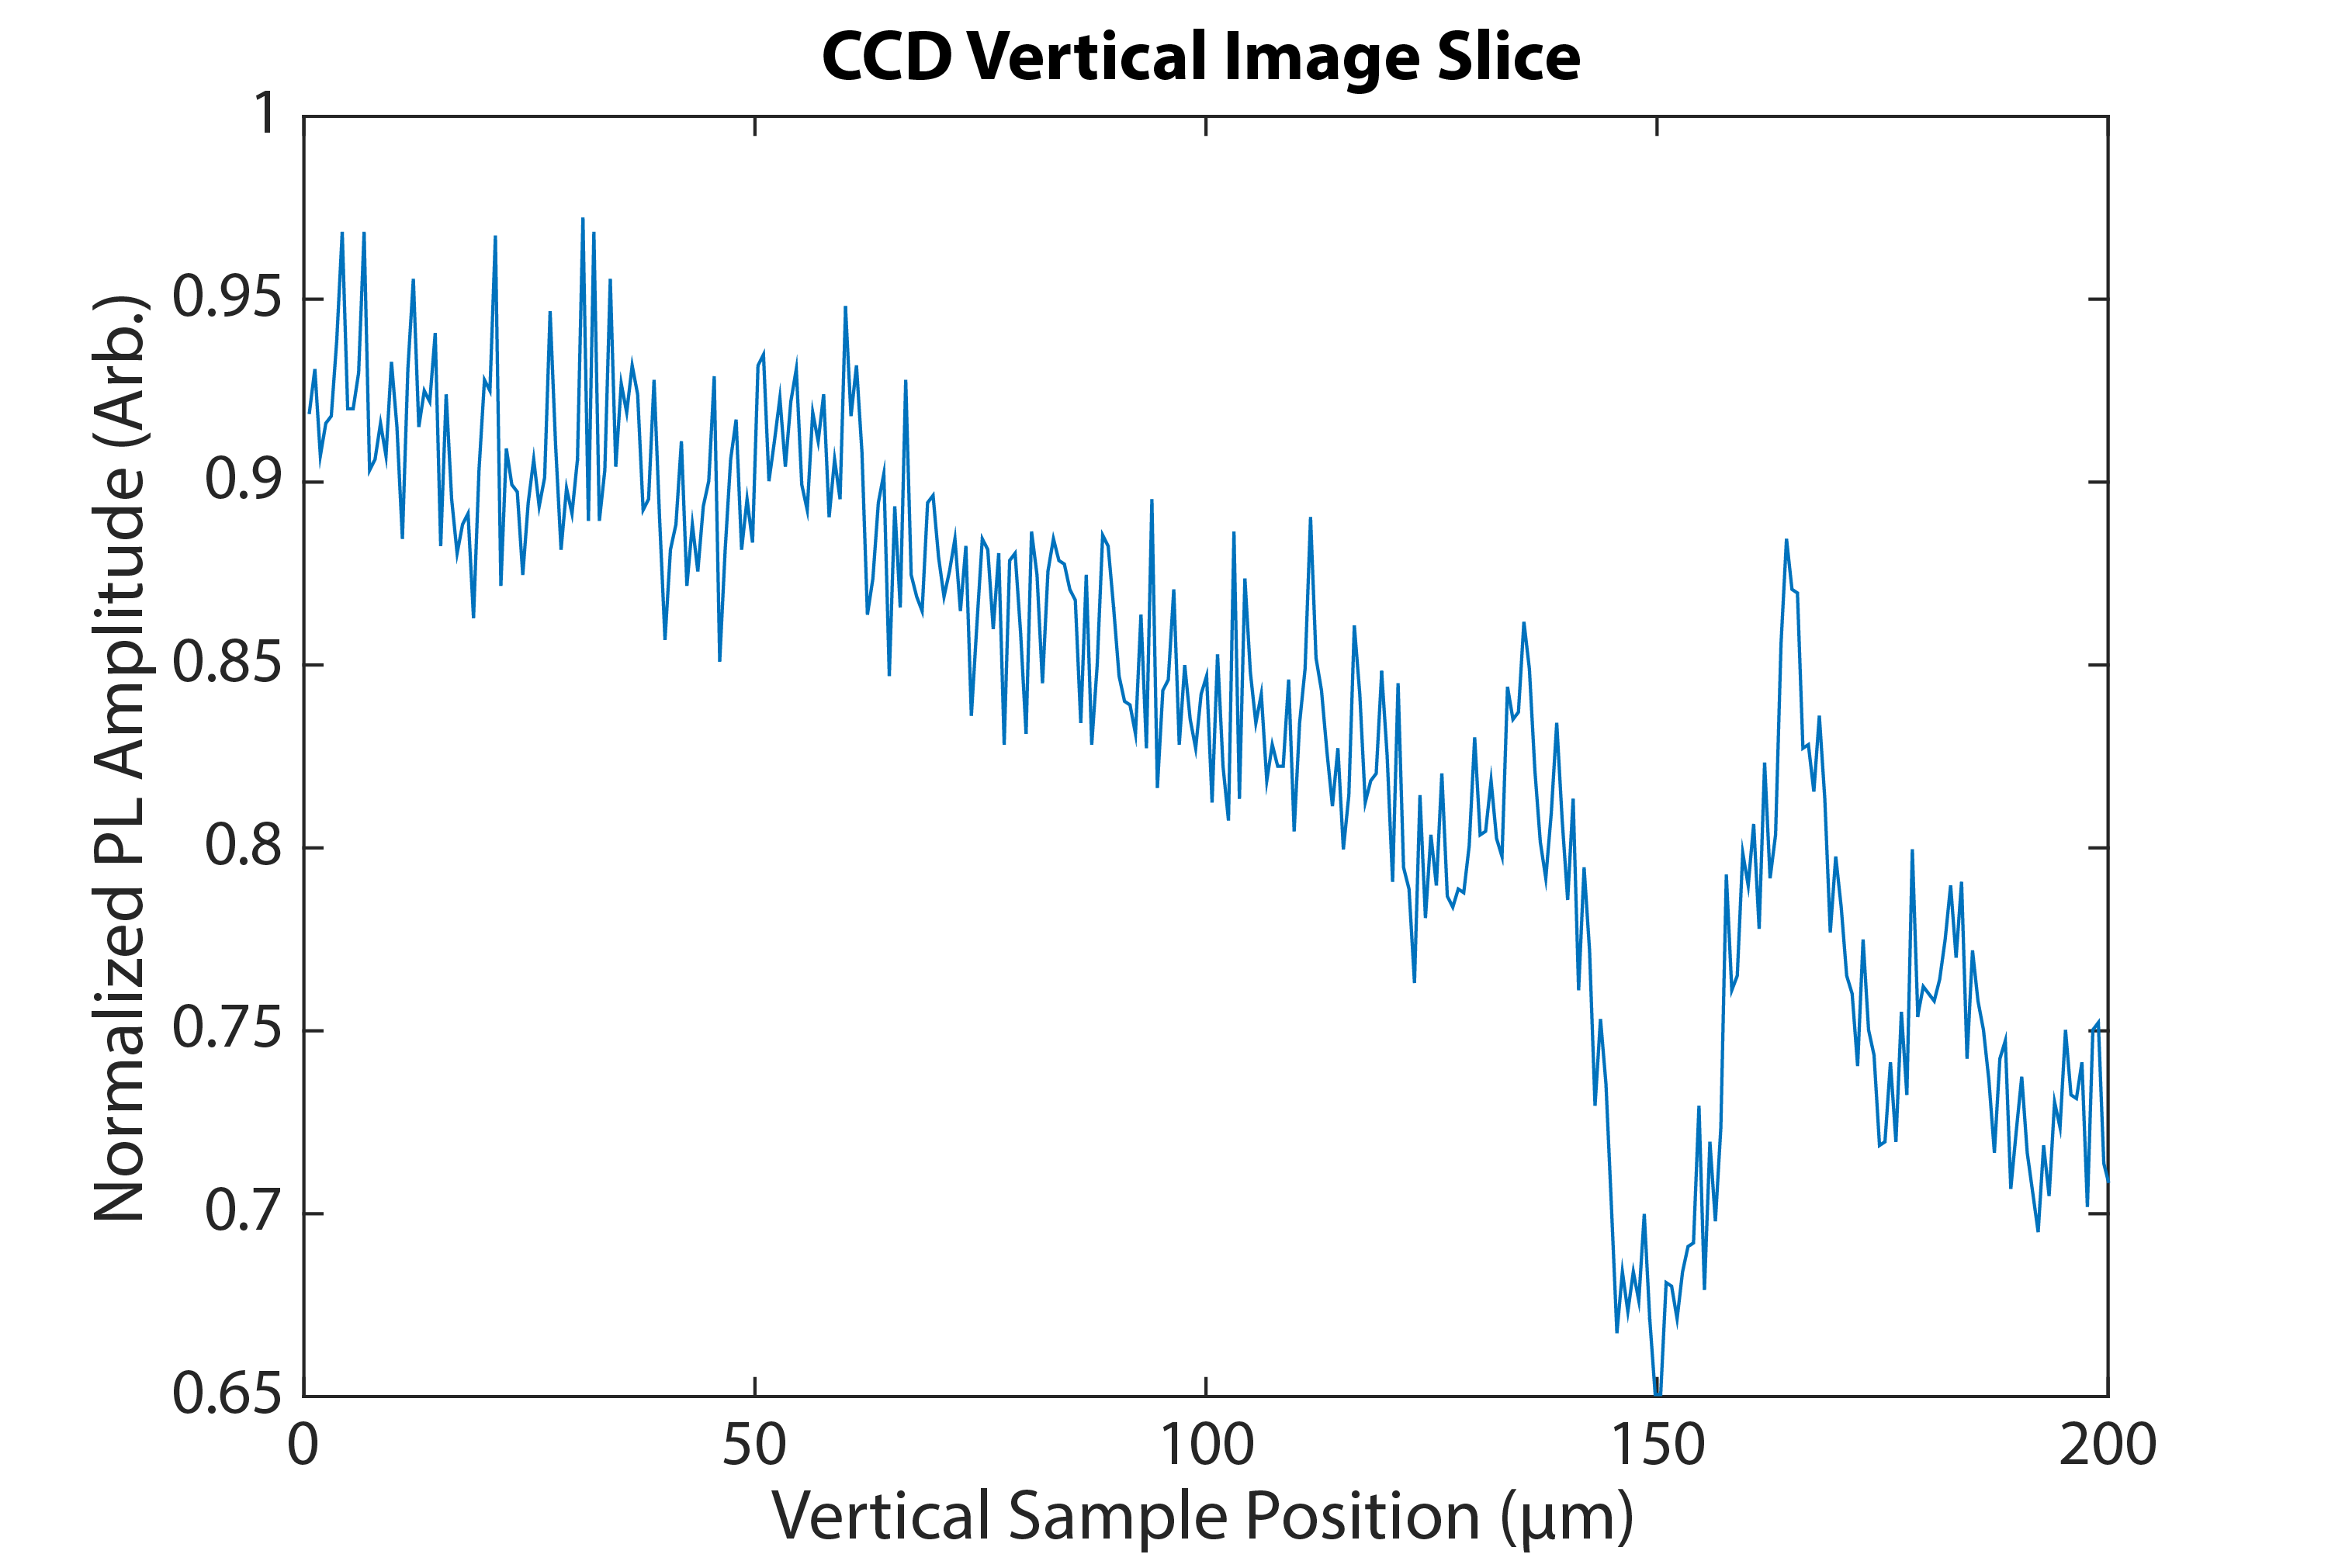
\includegraphics[width = .8\textwidth]{RawCCDIMGvertslce.png}
\caption{ \doublespacing A vertical 10QW PL amplitude slice from a CCD raw image. Effectively, these slices were stacked together along the lens translation axis to recover the second sample location axis and build a 3D surface of either PL amplitude or PL energy.}
\label{slice}
\end{figure}
\begin{figure}[h!]
\centering
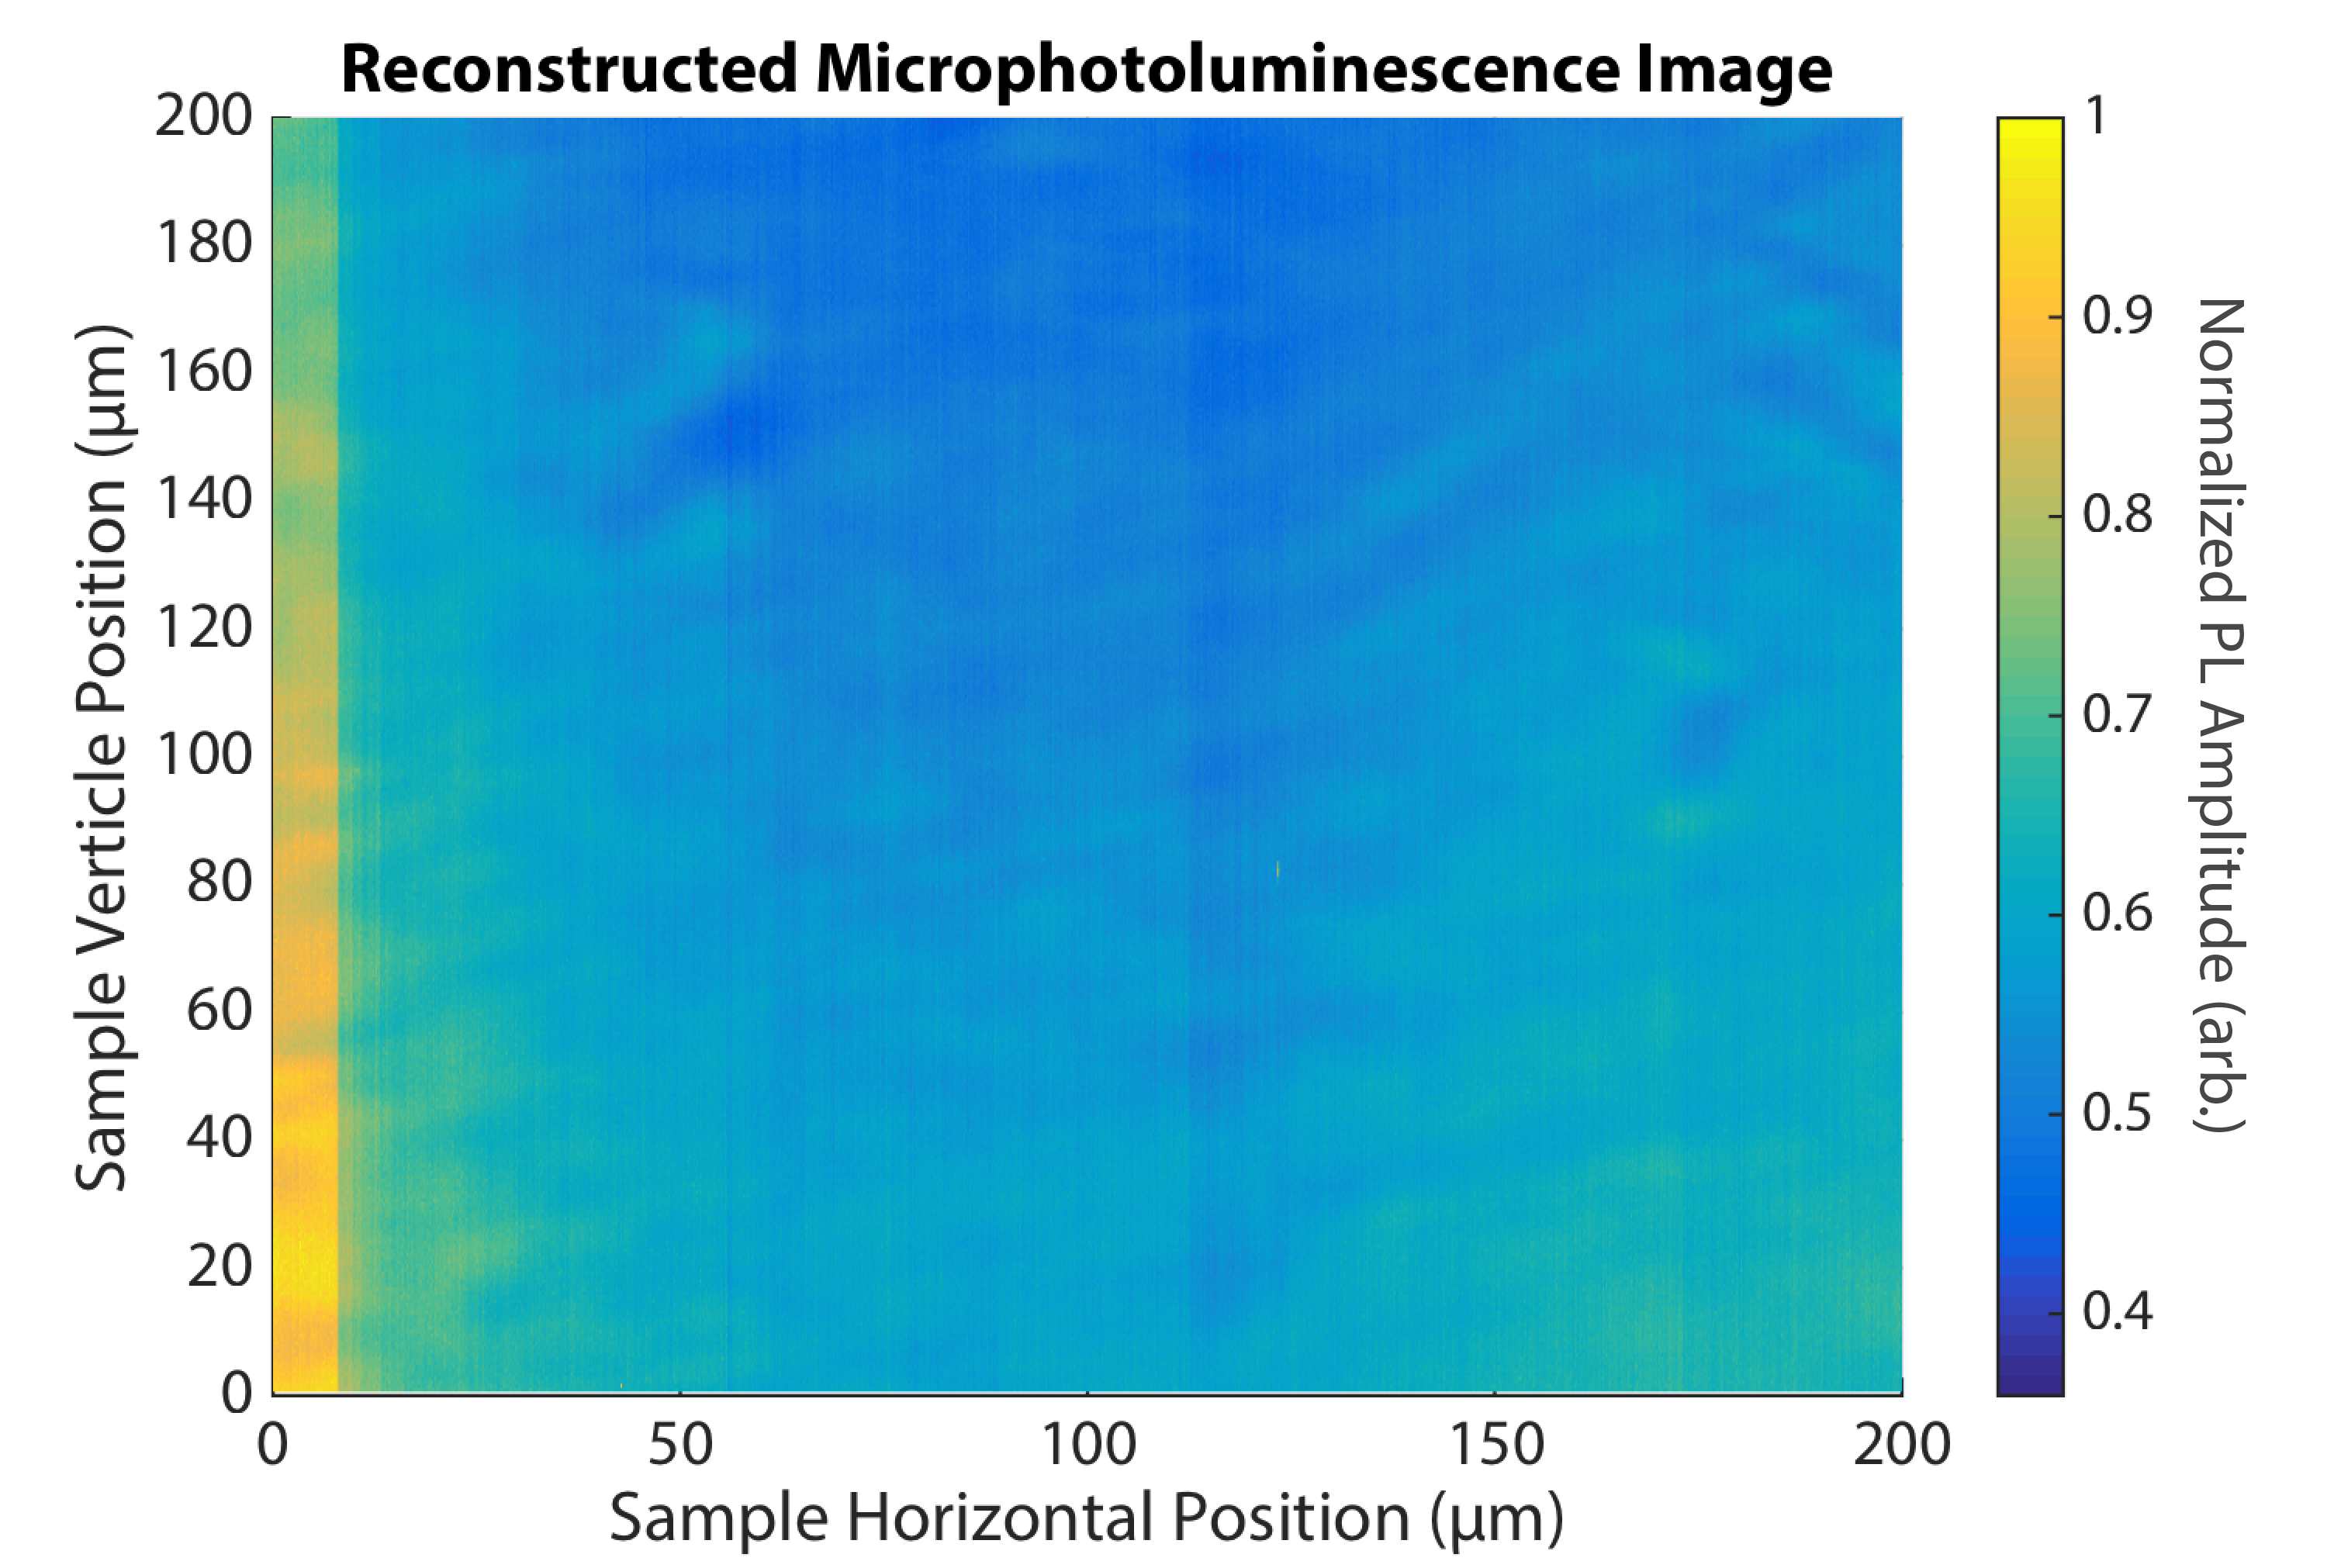
\includegraphics[width = .8\textwidth]{PLIMG_10QW.png}
\caption{ \doublespacing A reconstructed PL image of 10QW sample surface. The small features in the image correspond to striations and dust on the surface of the sample. The excitation spot's maximum intensity occurred near the bottom of the image, corresponding to the PL amplitude maximum.}
\label{total10qw}
\end{figure}
\indent From this image, we can estimate the resolution limit for the PL image alone. Doing so, we calculated that the resolution limit for our imaging system was limited by the repeatability of the lens position, $0.5\mu$m, which corresponds to 225nm at the sample surface. We were limited in the vertical direction by the pixel size, which was $13.6\mu$m. Our vertical resolution was no better than 612nm on the sample as a result. This was not our goal of 185nm; however, one can ameliorate this issue by inserting a telescope, with magnification two, between the NPBS and the achromatic doublet. An unfortunate side effect of increased resolution, however, was decreased signal strength. It was therefore necessary to increase CCD integration time or increase PL emission by increasing excitation power, but as we were exciting the sample with an already relatively high power of 1mW, increasing the resolution necessitated increasing integration time. For the 4QW sample, we took data with the telescope in place, but for the 10QW sample, a resolution of 225.0x612.0nm was the best we achieved.
 


\indent Though our resolution was less than optimal, we were still able to calculate an energy deviation map for the 10QW sample. To do this, we found the emission energy corresponding to the maximum PL amplitude at each vertical pixel. After doing this, we stacked each of these points (for which we had an energy vs. vertical sample position vector) along the horizontal image axis at each lens position. Once done, we then calculated the average PL energy for the entire PL image. Then, we found the local energy deviation from the average PL energy by subtracting the average PL energy from the local PL energy. Simply: 
\begin{equation}
\delta E_{i,j} = E_{i,j}-E_{avg}
\end{equation}
where $E_{avg}$ is the average emission energy for the whole PL picture, and $i,j$ index horizontal and vertical sample position respectively. Following this, we obtain our $\mu$PL map. However, this map is too noisy to see structure, as CCD intensity fluctuations of roughly 10 counts or 1\% of the total signal will affect which PL peak amplitude, and thus the peak energy at a given sample location location. Therefore, we must take our $\mu$PL energy deviation map and Gaussian smooth the energy deviation values by four to five pixels FWHM depending on the sample. Doing so, we obtain the energy deviation map seen in Figure \ref{devmap10QW}.

\begin{figure}[h!]
\centering
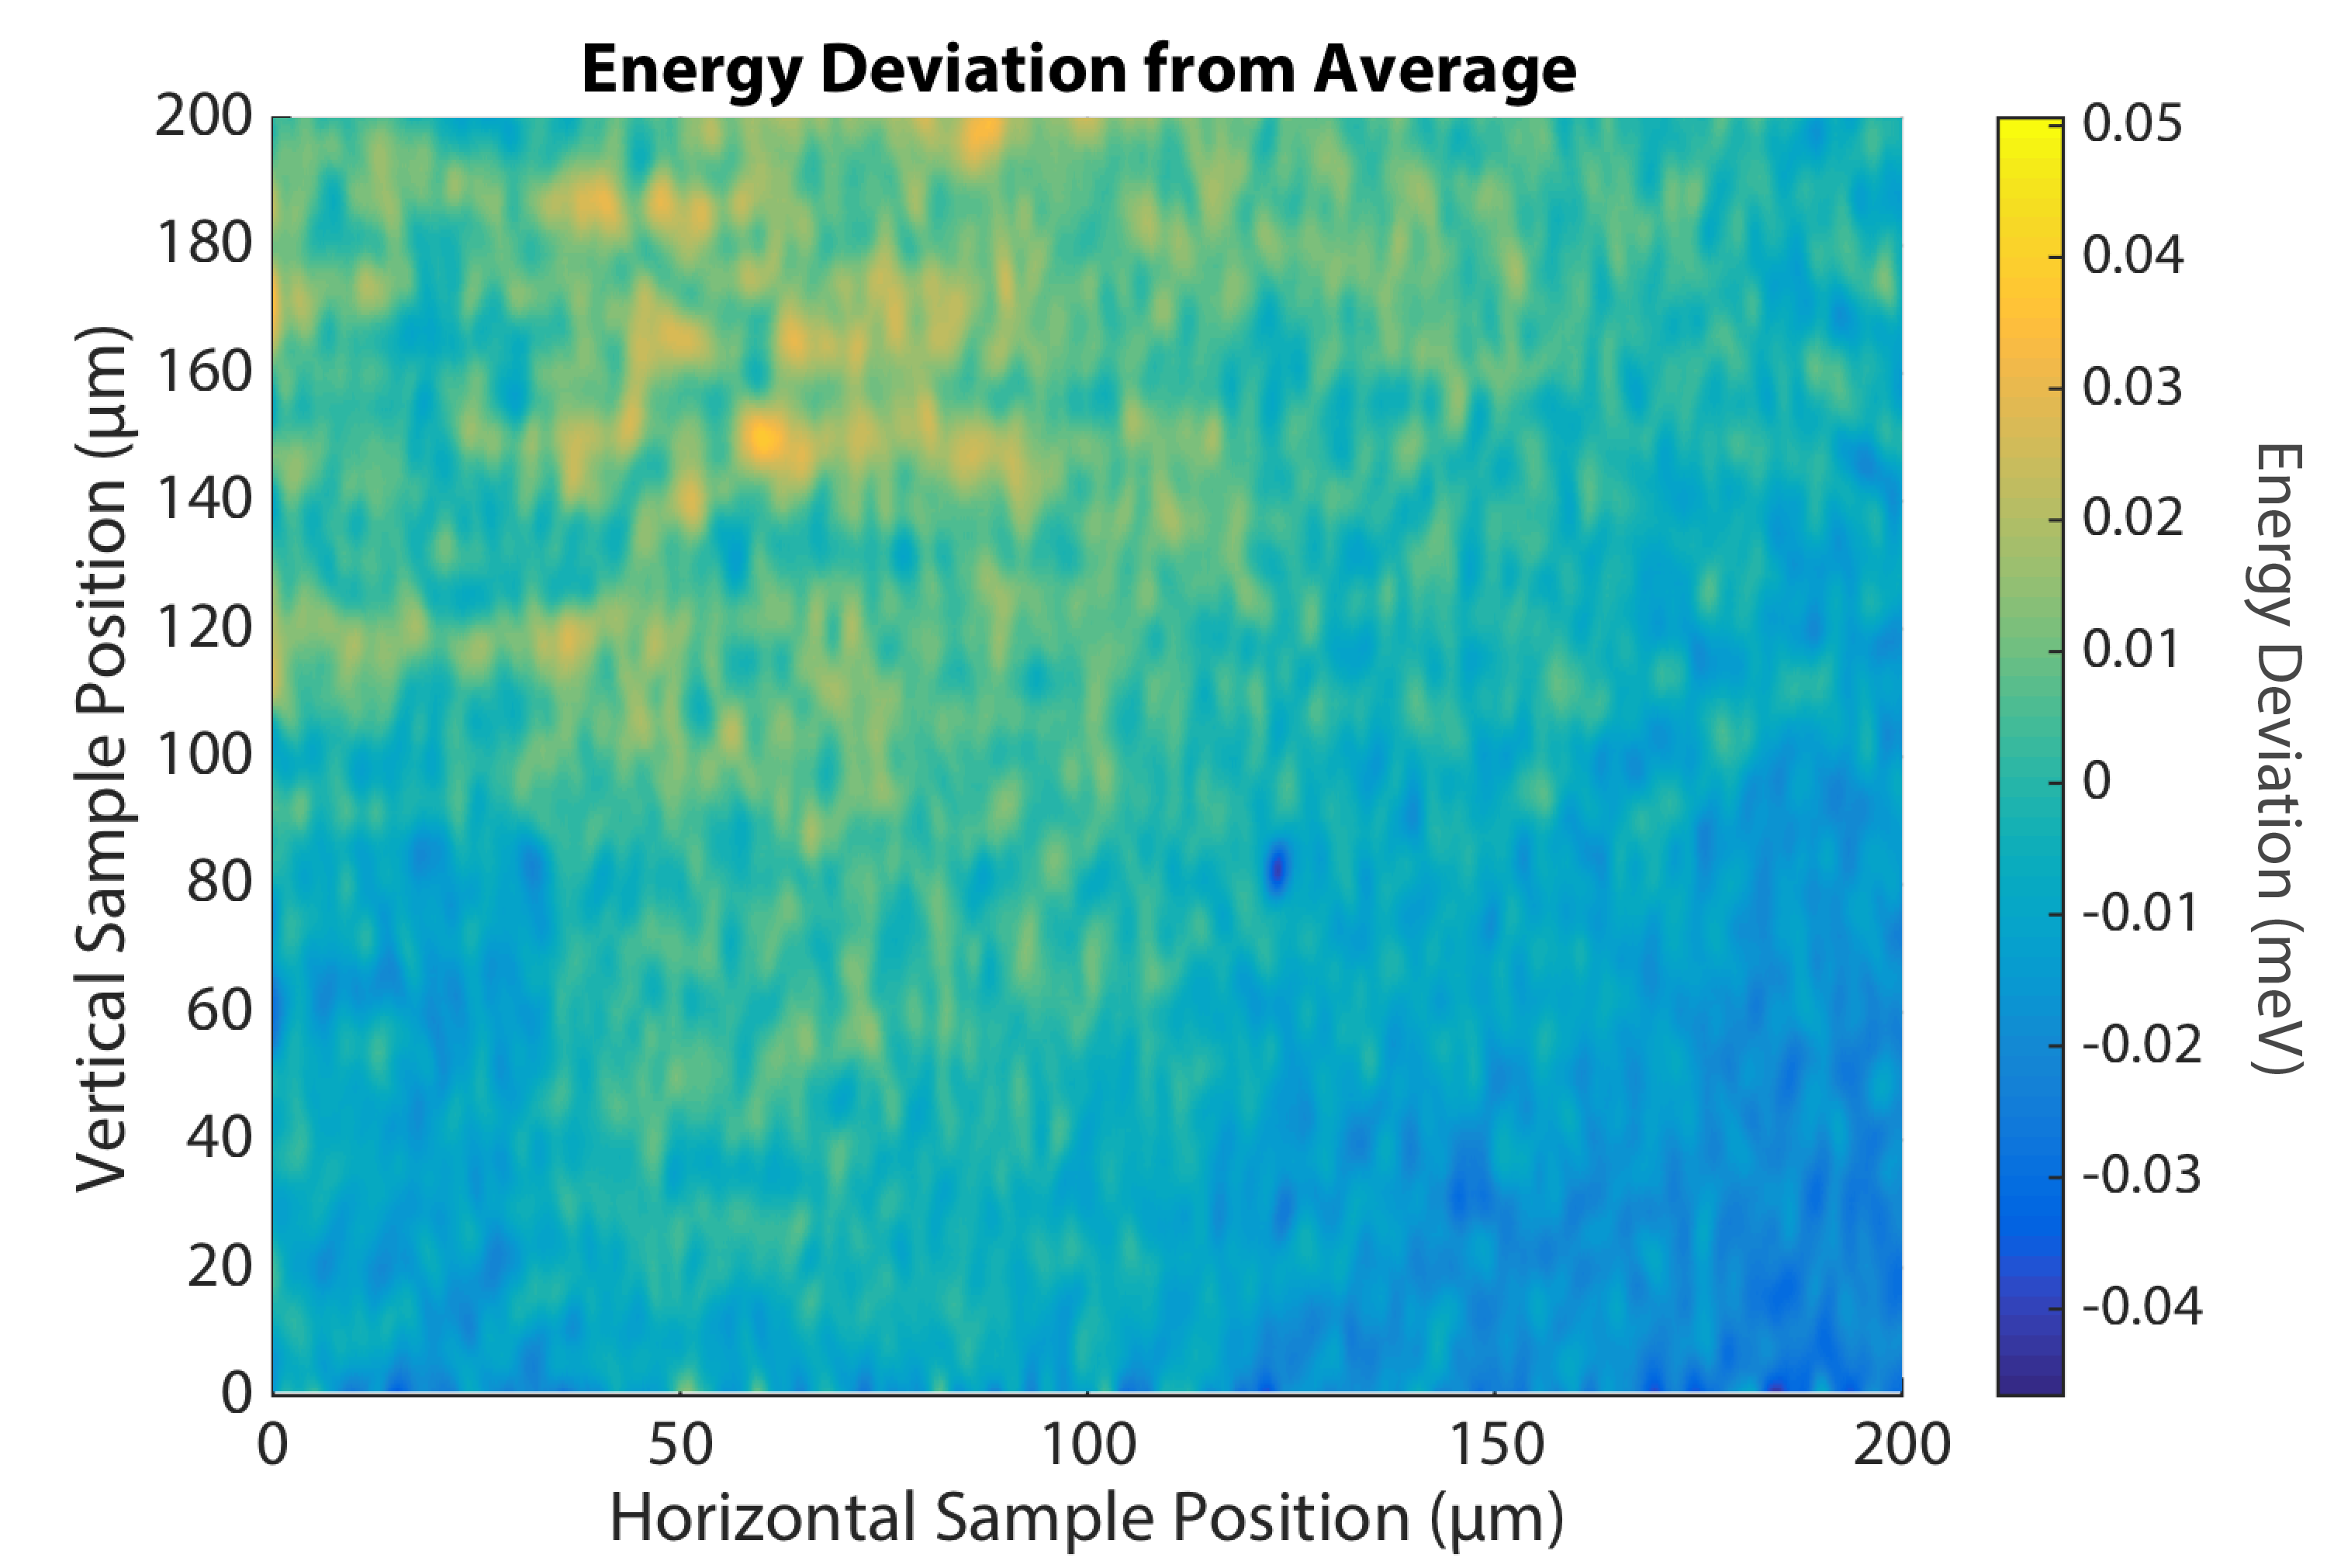
\includegraphics[width = .8\textwidth]{10QW_devplot.png}
\caption{ \doublespacing A $\mu$PL energy deviation image for the 10QW sample. Note the energy deviation we calculate is 0.1meV, peak to peak, at maximum.}
\label{devmap10QW}
\end{figure}

\newpage
\indent We expected energy deviations as a result of QW width fluctuations to behave according to the following equation:
\begin{equation}
\delta E = \frac{h^2 \pi^2}{2 \mu_{HH}}\Big ( \frac{1}{L^* \pm a}- \frac{1}{L^{*^2}} \Big )
\end{equation}
where $\delta E$ is the PL energy deviation due to a well width fluctuation of $\pm a$, $\mu_{HH}$ is the heavy-hole reduced mass, and $L^* = L+2\delta$ is the effective well width accounting for electron wave-function penetration of $15$\AA ~ into the AlGaAs barrier, and $\mu_{HH} = 0.055m_e$ is the reduced exciton mass CITE Glinka, Santos. 
\begin{itemize}
\item 10QW experiments\\
\* PL image and raw img, PL deviation small. Estimate smoothing, estimate resolution, comment on disorder agreement with thry.
\end{itemize}
\subsection{Disorder in a Four Quantum Well Structure}
\begin{itemize}
\item 4QW experiment\\
\* PL image and raw img, PL deviation slightly larger, but still small estimate, estimate rez, comment on disorder agreement with thry.
\end{itemize}
\subsection{Disorder in an Interfacial Quantum Dot Structure}
\begin{itemize}
\item IQD experiment\\
\* Introduce IQD, talk about disorder in IQD, show raw image, explain difference btwn IQD, MQW, estimate rez, comment on agreement with thry.
\end{itemize}
\section{PLE Results and Analysis}
\begin{itemize}
\item PLE curve analysis\\
show stock PLE curve, show slices, say what they mean, show peaks, say what peaks mean
\item PLE anti-stokes.
show anti-stokes t dep. curves\\
show anti-stokes pow-dep curves, talk about linearity or no, comment on CCD bs., \\
compare with thry, talk about mechanisms. well width dep
\item PLE stokes peak\\
show stokes pow-dep curves, talk about linearity or no, comment on CCD bs., \\
compare with thry, talk about well width dep, say mechanisms understood(?) point to lit chris and I found

\end{itemize}
